\documentclass[border=2mm]{standalone}
\usepackage{tikz}

\newcommand{\drawbox}[5]{
    \pgfmathsetmacro \angle {30}
    \pgfmathsetmacro \xd {{2/3*cos(\angle)}}
    \pgfmathsetmacro \yd {{2/3*sin(\angle)}}
    \pgfmathsetmacro \x {{#1-1+(#2-1)*(\xd)}}
    \pgfmathsetmacro \y {{#3-1+(#2-1)*(\yd)}}

    \draw[fill=#4] (\x,\y) -- (\x+1,\y) -- (\x+1,\y+1) -- (\x,\y+1) -- cycle;
    \draw[fill=#4] (\x,\y+1) -- (\x+\xd,\y+1+\yd) -- (\x+1+\xd,\y+1+\yd) -- (\x+1,\y+1) -- cycle;
    \draw[fill=#4] (\x+1,\y+1) -- (\x+1+\xd,\y+1+\yd) -- (\x+1+\xd,\y+\yd) -- (\x+1,\y) -- cycle;
    \node[fill=#4] at (\x+0.5,\y+0.5) {#5};

}

\begin{document}
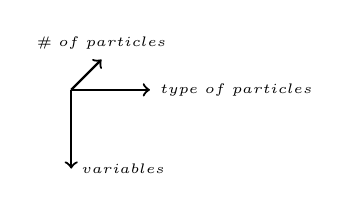
\begin{tikzpicture}[axis/.style={thick,->}]
    \coordinate (O) at (0, 0, 0);
    \draw[axis] (O) -- +(1, 0, 0) node [right] {\tiny{$type\ of\ particles$}};
    \draw[axis] (O) -- +(0, -1, 0) node [right] {\tiny{$variables$}};
    \draw[axis] (O) -- +(0, 0, -1) node [above] {\tiny{$\#\ of\ particles$}};
\end{tikzpicture}

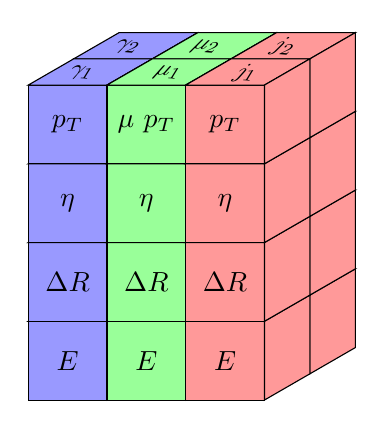
\begin{tikzpicture}

    \drawbox{1}{1}{1}{orange!70}{}
    \drawbox{1}{1}{2}{blue!40}{}
    \drawbox{1}{1}{3}{green!40}{}
    \drawbox{1}{1}{4}{blue!40}{}
    \drawbox{1}{0}{1}{blue!40}{$E$}
    \drawbox{1}{0}{2}{blue!40}{$\Delta R$}
    \drawbox{1}{0}{3}{blue!40}{$\eta$}
    \drawbox{1}{0}{4}{blue!40}{$p_T$}

    \drawbox{2}{1}{1}{green!40}{}
    \drawbox{2}{1}{2}{green!40}{}
    \drawbox{2}{1}{3}{green!40}{}
    \drawbox{2}{1}{4}{green!40}{}
    \drawbox{2}{0}{1}{green!40}{$E$}
    \drawbox{2}{0}{2}{green!40}{$\Delta R$}
    \drawbox{2}{0}{3}{green!40}{$\eta$}
    \drawbox{2}{0}{4}{green!40}{$\mu$ $p_T$}
    
    \drawbox{3}{1}{1}{red!40}{}
    \drawbox{3}{1}{2}{red!40}{}
    \drawbox{3}{1}{3}{red!40}{}
    \drawbox{3}{1}{4}{red!40}{}
     \drawbox{3}{0}{1}{red!40}{$E$}
    \drawbox{3}{0}{2}{red!40}{$\Delta R$}
    \drawbox{3}{0}{3}{red!40}{$\eta$}
    \drawbox{3}{0}{4}{red!40}{$p_T$}
    
    \node[rotate=-5, xslant=.5] at (0.1,3.82) {\footnotesize{$\gamma_1$}};
    \node[rotate=-5, xslant=.5] at (1.2,3.82) {\footnotesize{$\mu_{1}$}};
    \node[rotate=-5, xslant=.5] at (2.2,3.82) {\footnotesize{$j_{\tiny{1}}$}};

    \node[rotate=-5, xslant=.6] at (0.68,4.15) {\footnotesize{$\gamma_2$}};
    \node[rotate=-5, xslant=.6] at (1.68,4.15) {\footnotesize{$\mu_2$}};
    \node[rotate=-5, xslant=.6] at (2.68,4.15) {\footnotesize{$j_2$}};






\end{tikzpicture}
\end{document}
